\section{開発環境構築}
\subsection{Python3 環境構築}
\begin{frame}[shrink]
\frametitle{環境構築}
\framesubtitle{Python3}
  \begin{itemize}
\item Python を利用するためには各自の PC 上に環境を構築する必要があります
\item すでに python 開発環境を持っている人は以下の作業は不要です
\item 各状況に合わせて環境を作っていきます
    \begin{itemize}
\item Cloud で利用したい方は\href{https://www.pythonanywhere.com/}{\beamerbutton{https://www.pythonanywhere.com/}}で beginner account を作成(無料でインストール不要です)
\item Windows, Mac OSX, Linux で自分の PC に環境を作りたい方は\href{https://www.python.jp/install/install.html}{\beamerbutton{https://www.python.jp/}}を参照
    \end{itemize}
  \end{itemize}
\end{frame}
\begin{frame}[shrink,containsverbatim]
\frametitle{Pythonanywhere のアカウント開設}
  \begin{itemize}
\item ``Start running Python on line in less than a minute'' をクリック
  \end{itemize}
\includegraphics[width=1\textwidth]{../Figure/IL-figStartAnywhere.jpg}
\end{frame}
\begin{frame}[shrink,containsverbatim]
\frametitle{Pythonanywhere のアカウント作成}
  \begin{itemize}
\item ``Create a Biginner account'' をクリック
\item 無料のアカウントを作成します
  \end{itemize}
\includegraphics[width=1\textwidth]{../Figure/IL-figCreateAnywhereAccount.jpg}
\end{frame}
\begin{frame}[shrink,containsverbatim]
\frametitle{Pythonanywhere のアカウント登録}
  \begin{itemize}
\item ``Username'' を入力(任意)
\item ``Email'' を入力(m ドメイン以外でもかまいません)
\item ``Password'' を入力
\item ``I agree$\ldots$'' にチェック
\item ``Register'' をクリック
  \end{itemize}
\includegraphics[width=1\textwidth]{../Figure/IL-figAnywhereRegister.jpg}
\end{frame}
\begin{frame}[shrink,containsverbatim]
\frametitle{登録後の画面}
  \begin{itemize}
\item 登録アドレスにメイルが届くので確認
\item 以下のような画面が見えれば OK
  \end{itemize}
  \begin{itembox}{登録後の画面}
\includegraphics[width=1\textwidth]{../Figure/IL-figAnywhereDashboard.jpg}
  \end{itembox}
\end{frame}
\begin{frame}[shrink,containsverbatim]
\frametitle{自身の PC 上にインストールひと}
  \begin{itemize}
\item Idle を起動してください
  \end{itemize}
  \begin{columns}[t]
    \begin{column}{0.5\textwidth}
      \begin{itembox}{\footnotesize Mac, Linux のひと}
        \begin{itemize}
\scriptsize
\item ターミナルを起動して idle3 と入力
        \end{itemize}
        \begin{verbatim}
> idle3
        \end{verbatim}
      \end{itembox}
    \end{column}
    \begin{column}{0.5\textwidth}
      \begin{itembox}{\footnotesize Windows のひと}
        \begin{itemize}
\item スタートメニューから IDLE を起動
        \end{itemize}
      \end{itembox}
    \end{column}
  \end{columns}
\end{frame}
\begin{frame}[shrink,containsverbatim]
\frametitle{開発統合環境}
\framesubtitle{IDLE と Pythonanywhere}
  \begin{itemize}
\item Mac, Windows, Linux の人もこれで準備ができました
\item それぞれ以下のような画面が見えるはずです
\item 以後,いずれかの開発統合環境を利用していきます
\item Pythonanywhere や IDLE は編集,実行が統合された環境を提供しています
\item IDLE の使い方は\href{https://docs.python.org/ja/3/library/idle.html?highlight=idle}{\beamerbutton{Python 公式}}を参照
    \begin{itemize}
\item \href{http://www.isc.meiji.ac.jp/~mizutani/python/intro1_python.html}{\beamerbutton{http://www.isc.meiji.ac.jp/~mizutani/python/intro1\_python.html}}も参考になるかも
    \end{itemize}
  \end{itemize}
  \begin{columns}[c]
    \begin{column}{5cm}
\includegraphics[width=1\textwidth]{../Figure/IL-figIDLE.jpg}
    \end{column}
    \begin{column}{5cm}
\includegraphics[width=1\textwidth]{../Figure/IL-figPythonanywhere.jpg}
    \end{column}
  \end{columns}
\end{frame}
\subsection{動作確認}
\begin{frame}[shrink,containsverbatim]
\frametitle{開発環境テスト用コード}
%\vspace{-2zw}
%  \begin{lstlisting}[caption={環境テスト用コード},label=lst:test,numbers=none]
%import matplotlib.pyplot as plt
%print('Hello World')
%plt.plot([1, 2, 3, 4])
%plt.show()
%  \end{lstlisting}
  \begin{itemize}
\item \href{https://sites.google.com/a/presystems.xyz/sample/home/elementary-computer-science}{\beamerbutton{https://sites.google.com/a/presystems.xyz/sample/home/elementary-computer-science}} 
からhello.pyをダウンロード
  \end{itemize}
\vspace{-1em}
  \begin{columns}[t]
    \begin{column}{0.5\textwidth}
      \begin{itembox}{\footnotesize IDLE 利用のひと}
        \begin{itemize}
\scriptsize
\item File->Open で hello.py を開く
        \end{itemize}
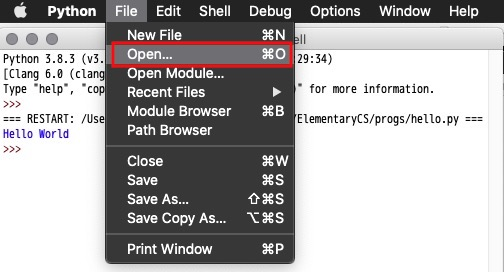
\includegraphics[width=1\textwidth]{./Figure/elementaryCS-figOpenFile.jpg}
      \end{itembox}
    \end{column}
    \begin{column}{0.5\textwidth}
      \begin{itembox}{\footnotesize Pythonanywhere 利用のひと}
\scriptsize
        \begin{itemize}
\item 右上 ``Files'' をクリック
\item ''upload'' をクリックして hello.py をアップロード
\item hello.py をクリックすると中が見れます
        \end{itemize}
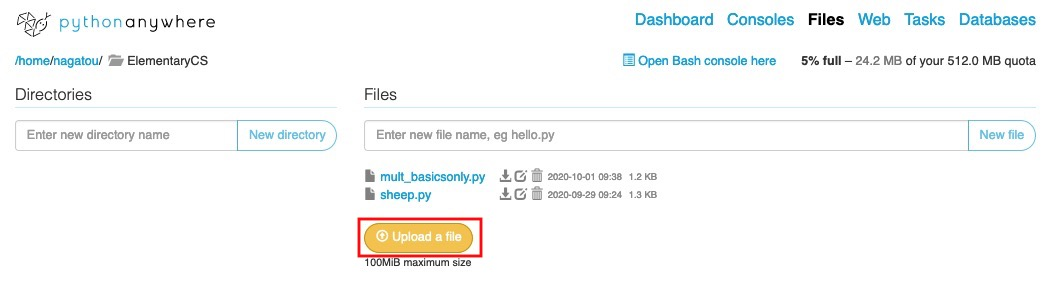
\includegraphics[width=1\textwidth]{./Figure/elementaryCS-figUpload.jpg}
      \end{itembox}
    \end{column}
  \end{columns}
\end{frame}
\begin{frame}[shrink,containsverbatim]
\frametitle{プログラムの実行}
%  \begin{itemize}
%\item \href{https://sites.google.com/a/presystems.xyz/sample/home/information-literacy}{\beamerbutton{https://sites.google.com/a/presystems.xyz/sample/home/information-literacy}}から test.py をダウンロード
%  \end{itemize}
  \begin{columns}[t]
    \begin{column}{0.5\textwidth}
      \begin{itembox}{\footnotesize IDLE 利用のひと}
        \begin{itemize}
\scriptsize
\item Run->Run Module をクリック
\item ``Hello World'' が表示されれば正常
        \end{itemize}
\includegraphics[width=1\textwidth]{../Figure/IL-figTestIDLE.jpg}
      \end{itembox}
    \end{column}
    \begin{column}{0.5\textwidth}
      \begin{itembox}{\footnotesize Pythonanywhere 利用のひと}
\scriptsize
        \begin{itemize}
\item Run this file をクリック
\item 下半分の黒い画面に ``Hello World'' と表示されれば正常
\item 下半分の黒い画面で exit() と入力してください
        \end{itemize}
\includegraphics[width=1\textwidth]{../Figure/IL-figTestCloud.jpg}
      \end{itembox}
    \end{column}
  \end{columns}
\end{frame}
